\documentclass[11pt]{beamer}\usepackage[]{graphicx}\usepackage[]{color}
% maxwidth is the original width if it is less than linewidth
% otherwise use linewidth (to make sure the graphics do not exceed the margin)
\makeatletter
\def\maxwidth{ %
  \ifdim\Gin@nat@width>\linewidth
    \linewidth
  \else
    \Gin@nat@width
  \fi
}
\makeatother

\definecolor{fgcolor}{rgb}{0.345, 0.345, 0.345}
\newcommand{\hlnum}[1]{\textcolor[rgb]{0.686,0.059,0.569}{#1}}%
\newcommand{\hlstr}[1]{\textcolor[rgb]{0.192,0.494,0.8}{#1}}%
\newcommand{\hlcom}[1]{\textcolor[rgb]{0.678,0.584,0.686}{\textit{#1}}}%
\newcommand{\hlopt}[1]{\textcolor[rgb]{0,0,0}{#1}}%
\newcommand{\hlstd}[1]{\textcolor[rgb]{0.345,0.345,0.345}{#1}}%
\newcommand{\hlkwa}[1]{\textcolor[rgb]{0.161,0.373,0.58}{\textbf{#1}}}%
\newcommand{\hlkwb}[1]{\textcolor[rgb]{0.69,0.353,0.396}{#1}}%
\newcommand{\hlkwc}[1]{\textcolor[rgb]{0.333,0.667,0.333}{#1}}%
\newcommand{\hlkwd}[1]{\textcolor[rgb]{0.737,0.353,0.396}{\textbf{#1}}}%
\let\hlipl\hlkwb

\usepackage{framed}
\makeatletter
\newenvironment{kframe}{%
 \def\at@end@of@kframe{}%
 \ifinner\ifhmode%
  \def\at@end@of@kframe{\end{minipage}}%
  \begin{minipage}{\columnwidth}%
 \fi\fi%
 \def\FrameCommand##1{\hskip\@totalleftmargin \hskip-\fboxsep
 \colorbox{shadecolor}{##1}\hskip-\fboxsep
     % There is no \\@totalrightmargin, so:
     \hskip-\linewidth \hskip-\@totalleftmargin \hskip\columnwidth}%
 \MakeFramed {\advance\hsize-\width
   \@totalleftmargin\z@ \linewidth\hsize
   \@setminipage}}%
 {\par\unskip\endMakeFramed%
 \at@end@of@kframe}
\makeatother

\definecolor{shadecolor}{rgb}{.97, .97, .97}
\definecolor{messagecolor}{rgb}{0, 0, 0}
\definecolor{warningcolor}{rgb}{1, 0, 1}
\definecolor{errorcolor}{rgb}{1, 0, 0}
\newenvironment{knitrout}{}{} % an empty environment to be redefined in TeX

\usepackage{alltt}
\usepackage{amsmath}
\usepackage{amssymb}
\usepackage{geometry}
\usepackage{graphicx}
\usepackage{url}
\IfFileExists{upquote.sty}{\usepackage{upquote}}{}
\begin{document}

\begin{frame}
\large
Lecture 13:\\
Inference for Simple Linear Regression\\
STAT 310, Spring 2021
\end{frame}

%---------------------------
\begin{frame}
A \textbf{parameter} is a numerical characteristic of a population (e.g., the population mean height $\mu$ of all students at CSUEB)\\
\vspace{15pt}

\textbf{Statistical inference} refers to the process of using data collected from a sample to answer questions about population parameters.
\vspace{2pt}
\begin{itemize}
\item \textbf{Point estimate}: our best guess for the value of the population parameter (e.g., the sample mean height $\bar{x}$ of $n=100$ randomly selected CSUEB students)
\vspace{5pt}
\item \textbf{Confidence interval}: a plausible range of values for the population parameter
\vspace{5pt}
\item \textbf{Hypothesis test}: is a specific value of the population parameter plausible?
\end{itemize}
\end{frame}

%---------------------------
\begin{frame}
\textbf{Simple linear regression model for the population}:\\
$$ y = \beta_0 + \beta_1 x + \epsilon $$\\
$\beta_0$ and $\beta_1$ are the population parameters (fixed and unkown)\\
\vspace{30pt}

\textbf{Least squares line (estimated from the sample)}:\\
$$ \hat{y} = \hat{\beta}_0 + \hat{\beta}_1 x $$\\
$\hat{\beta}_0$ and $\hat{\beta}_1$ are the estimates (varies from sample to sample)\\
\end{frame}

%---------------------------
\begin{frame}
\end{frame}

%---------------------------
\begin{frame}
%\vspace{-1cm}
Confidence interval for the slope $\beta_1$:
$$\hat{\beta}_1 \pm t^* SE_{\hat{\beta}_1}$$

\begin{itemize}
\item $\hat{\beta}_1$ is the point estimate 
\item $t^*$ is the t-critical value, which depends on the confidence level and has $n-2$ degrees of freedom
\item $SE_{\hat{\beta}_1}$ is the standard error of the slope estimate 
\end{itemize}
\end{frame}

\begin{frame}
%\vspace{-1cm}
Hypothesis test for whether or not the slope parameter $\beta_1$ is different than zero.  We can also interpret this as a hypothesis test for whether or not there is a linear association between $x$ and $y$.\\
\vspace{10pt}
$H_0: \beta_1 = 0$\\
\vspace{5pt}
$H_A: \beta_1 \neq 0$\\
\vspace{10pt}
Test statistic:\\
$$t = \frac{\hat{\beta}_1}{SE_{\hat{\beta}_1}}; \quad \text{df=n-2}$$\\
\vspace{10pt}

The test statistic is then used to compute the $p$-value.  When using the default significance level ($\alpha = 0.05$), we would reject $H_0$ when the $p$-value $<0.05$.
\end{frame}

\begin{frame}[fragile]{Example}
Let's go back to the example of using a student's high school GPA ($x$) to predict their college GPA ($y$).  Shown below is a scatterplot of the data, and the output from fitting this simple linear regression model in R.

\scriptsize
\begin{verbatim}
Coefficients:
            Estimate Std. Error t value Pr(>|t|)    
(Intercept)   0.2168     0.3250   0.667    0.506    
hs_gpa        0.7091     0.1003   7.069 5.73e-11 ***
---
Signif. codes:  0 ‘***’ 0.001 ‘**’ 0.01 ‘*’ 0.05 ‘.’ 0.1 ‘ ’ 1
\end{verbatim}

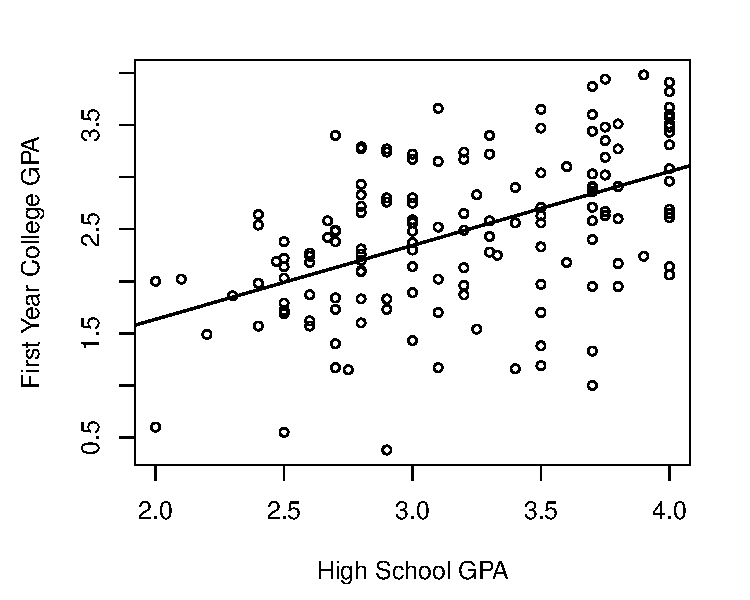
\includegraphics[scale=0.3]{figure/gpa_scatter_line.pdf}
\end{frame}

\begin{frame}{Example}
(a) Do the data provide strong evidence of a linear association between high school GPA and first-year college GPA?  State the null and alternative hypothesis, report the test statistic and $p$-value, and state your conclusion.
\vspace{5cm}
\end{frame}

\begin{frame}{Example}
(b) Calculate a 95\% confidence interval for the slope parameter $\beta_1$.  Note that there are $n=150$ students in this data set.
\vspace{6cm}
\end{frame}

%------------------------------------------------------
\begin{frame}{Conditions for Simple Linear Regression}

\begin{itemize}
\item \textbf{Linearity}.  The data should follow a linear trend.
\vspace{5pt}
\item \textbf{Constant variability}.  The variability of the points around the least squares line remains roughly constant.
\vspace{5pt}
\item \textbf{Normality}.  The residuals should be approximately normally distributed with mean 0.
\vspace{5pt}
\item \textbf{Independence}.  Values of the response variable are independent of each other. 
\end{itemize}
\end{frame}

\begin{frame}{Residual Plots}
\begin{itemize}
\item One useful way to check the conditions is to look at a plot of the residuals, $\hat{e}_i = y_i - \hat{y}_i$, versus the predictor, $x_i$.
\vspace{5pt}
\item One purpose of residual plots is to identify characteristics or patterns still apparent in the data after fitting the model.
\vspace{5pt}
\item Residual plots are especially useful for checking the constant variability condition.
\vspace{5pt}
\item Ideally, the residual plot should show no obvious pattern, and the points are randomly scattered around 0.
\end{itemize}
\end{frame}

\begin{frame}{Example: Residual Plot}
For the simple linear regression model between high school and first year college GPA, the points in the residual plot look randomly scattered around the horizontal line at 0.  This indicates that the condition of constant variability is met.
\begin{figure}
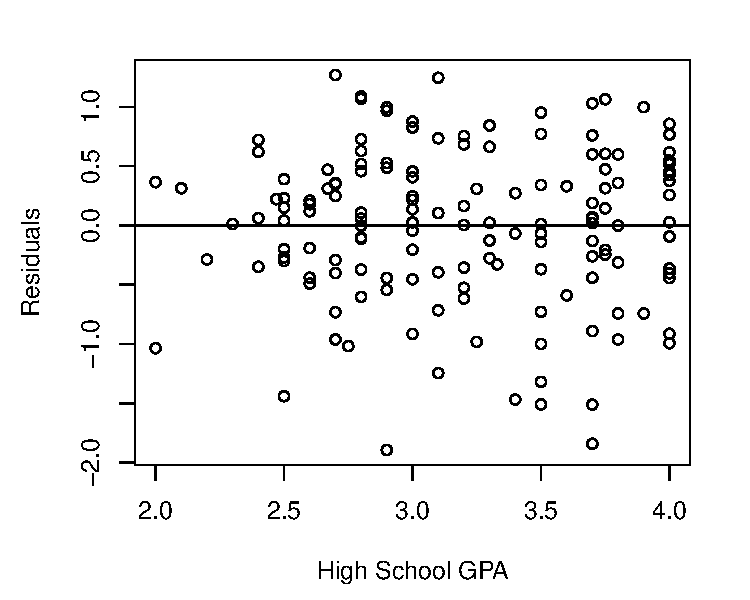
\includegraphics[scale=0.5]{figure/gpa_resid.pdf}
\end{figure}
\end{frame}

\begin{frame}{Example: Normality of Residuals}
To check whether the the residuals are normally distributed we can make a histogram.  The histogram should be symmetric about 0 and have an approximate bell-curve shape.  For the GPA example, the residuals appear to have an approximate normal distribution, and there are no outliers.
\begin{figure}
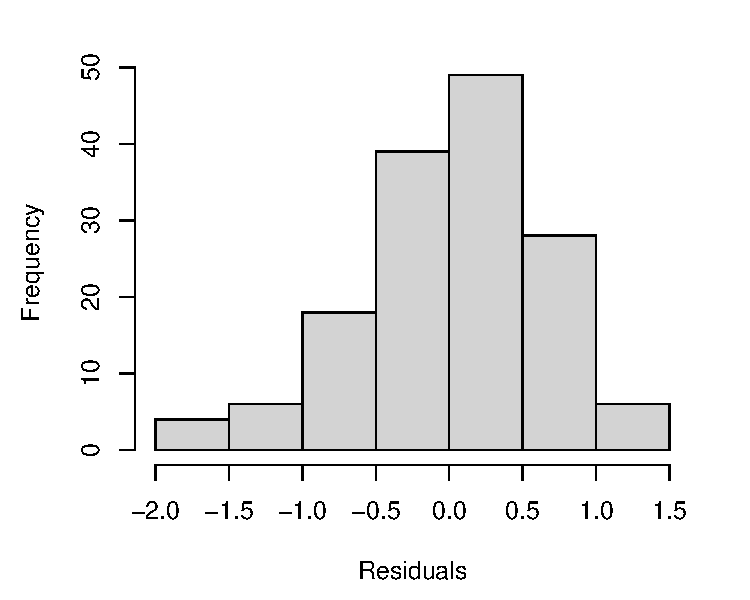
\includegraphics[scale=0.5]{figure/hist_resid.pdf}
\end{figure}
\end{frame}

\begin{frame}{Example: Nonconstant variability}
An example of a violation of the constant variability condition. This residual plot shows a \textbf{fan pattern}.
\begin{figure}
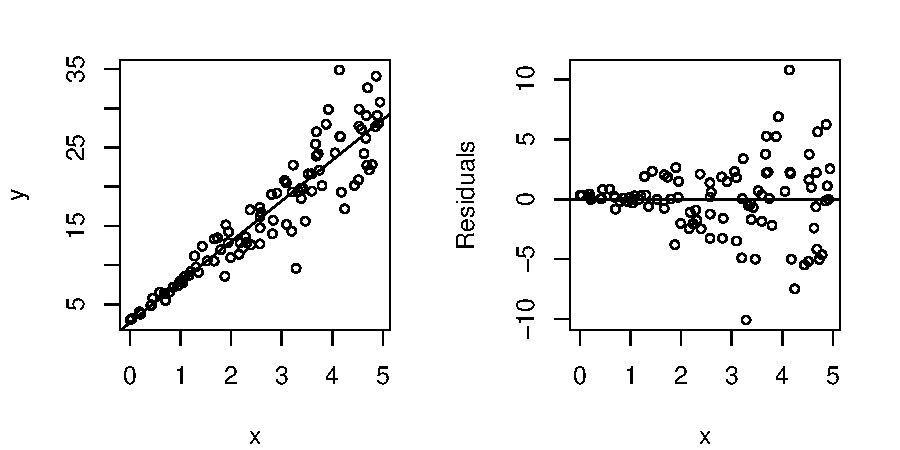
\includegraphics[scale=0.65]{figure/resid_var.pdf}
\end{figure}
\end{frame}

\begin{frame}{Example: Nonlinearity}
An example of a violation of the linearity condition.
\begin{figure}
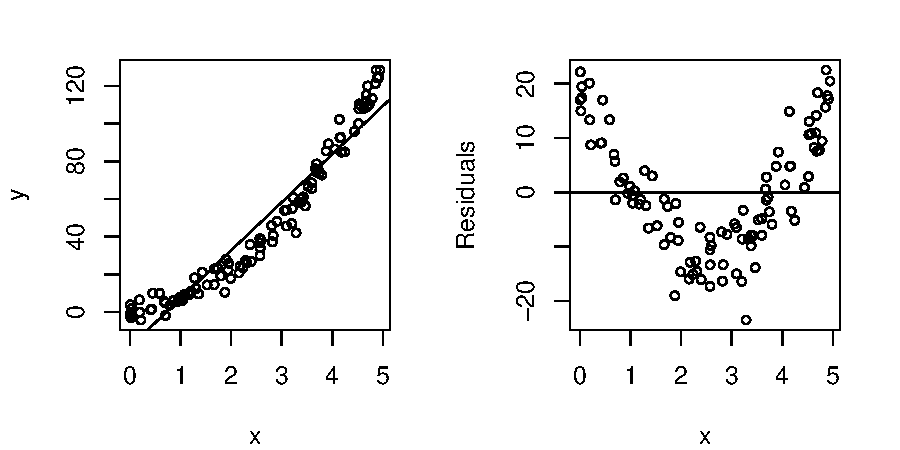
\includegraphics[scale=0.65]{figure/resid_nonlin.pdf}
\end{figure}
\end{frame}

% \begin{frame}[fragile]{Example: Slope Not Significant}
% In case you are wondering, here is an example of a scatterplot where the slope $\beta_1$ of the regression line is \textbf{not} significantly different than 0.  As you can see, there does not appear to be a linear association between $x$ and $y$.  
% \small
% \begin{verbatim}
% Coefficients:
%             Estimate Std. Error t value Pr(>|t|)
% (Intercept)  0.01145    0.07929   0.144    0.885
% x           -0.10537    0.07807  -1.350    0.180
% \end{verbatim}
% \begin{figure}
% 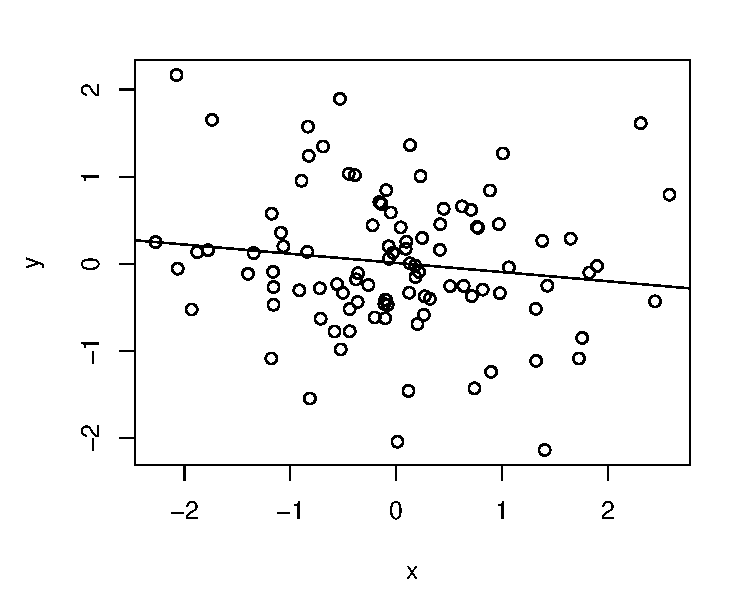
\includegraphics[scale=0.4]{figure/scatter_slope_zero.pdf}
% \end{figure}08
% \end{frame}

\end{document}
